\chapter{\ifenglish Background Knowledge and Theory\else ทฤษฎีที่เกี่ยวข้อง\fi}

In order to create the AI, we first need to implement \RootOurs{}. This requires knowledge of game programming fundamentals and extensive knowledge of the rules of \RootB{}. However, there are minor rule differences between \RootV{} and \RootB{}. Since \RootV{}`s AIs are the root cause of our project, we also need to find and implement these minor differences in our \RootOurs{}.

The next step is to implement \RootAI{}, the framework for running \RootOurs{} and training AI agents. There are two AI agent implementation methods that require additional self-study: Monte Carlo tree search and reinforcement learning neural networks.

\section{Root}
Root is an \textbf{asymetric game}: a game where each player starts with different setups, gameplay mechanics, etc. \cite{Mike_Shor-2023-10-06}. Although Root's base actions, such as move and battle, are the same for every faction, each faction starts differently, and each has its own unique mechanics and rules. Thus, Root sits closer to the asymmetric side in the symmetric-asymmetric spectrum. \\
Examples of symmetric games are Chess, Monopoly, Prisoner's Dilemma, etc.\\
Examples of other asymmetric games are Tapestry, Dune, Cthulhu Wars, etc.

Root is an \textbf{imperfect information game}: a game where there is information hidden from the player \cite{osborne1994course}. Most elements of Root, such as warrior placement, building count, etc., are laid out for all players to see. But cards on the player's hand are only visible to that player, i.e., other players' cards in hand are the hidden information in this game.

Root is a \textbf{non-deterministic game}: a game where there is some element of randomness involved, such as rolling dice or shuffling cards. Root has both, rolling dice in battle and drawing cards from a shuffled draw pile.

\subsection{Brief Rules of Root} \label{brief-rules-of-root}

Root is a turn-based game for 2-4 players in which you fight as one of four factions against other factions to take control of the ``Woodland''.

The rule is simple: The player who scores 30 victory points or plays the dominance card and fulfills its condition (the card that changes the endgame win condition) first wins. The players play on the map of Woodland (Figure \ref{fig:root-game-board}), which contains 12 clearings, each with different suits and a different number of slots for building. There are also paths that connect those clearings, moving warriors from one clearing to another.

\begin{figure}
  \begin{center}
    \includegraphics[width=\textwidth]{root_game_board.jpg}
  \end{center}
  \caption{Woodland, Root's game board}
  \label{fig:root-game-board}
\end{figure}

Each player will take his turn throughout three phases: birdsong, daylight, and evening. The player will be instructed on what he must do and what actions he can take in each phase. Also, each faction will have special abilities that can be used during their turn. Instructions and actions will vary from faction to faction, but there are actions that are shared by all factions, called key actions. There are three key actions:

\begin{enumerate}
  \item \textbf{Move}: Take any number of your warriors from one clearing and move them to one adjacent clearing.
  \item \textbf{Craft}: Using crafting pieces you have to craft a card from your hand. After crafting, gain benefits or effects on the crafted card.
  \item \textbf{Battle}: Choose a clearing where you have warriors as the clearing of battle. You are the attacker. Choose another player in the clearing of battle to be the defender. Roll two dice. The attacker deals hits equal to the higher roll, and the defender deals hits equal to the lower roll. Both players deal hits simultaneously and remove pieces equal to the number of hits they receive.
\end{enumerate}

Other than key actions, there will be some specific actions belonging to each faction. We will describe them in detail with an explanation of how each phase of each faction works in Tables \ref{tab:marquise-flow} and \ref{tab:eyrie-flow}.

Some of the rules will not be explained here, as they are not crucial or essential. For more details on rules, see \cite{RootBoardGameRules}.

\renewcommand{\arraystretch}{1.5}

% \afterpage{
  % \begin{landscape}
\begin{table}
  \caption{\Marquise{} Flow}
  \label{tab:marquise-flow}
  \centering
  \resizebox{\textwidth}{!}{\begin{tabular}{|p{3cm}|p{9cm}|p{4cm}|} 
    \hline
    \multicolumn{3}{|c|}{\Marquise} \\
    \hline
    Birdsong & Daylight & Evening \\ 
    \hline
    \tabitem Place one wood token at each sawmill. 
  & \tabitem Craft any cards in your hand using workshops.

    \tabitem Take up to three of the following actions (plus one per bird suit card you spend): 
    
      \tabsubitem Battle

      \tabsubitem March: Takes two moves

      \tabsubitem Recruit: Place one warrior at each recruiter.

      \tabsubitem Build: Place one building in a clearing you rule by spending wood tokens equal to its cost.

      \tabsubitem Overwork: Spend a card to place one wood token at one sawmill in a clearing whose suit matches the card spent.
  & \tabitem Draw one card plus one card per draw bonus. (Discard down to five if you have more than five cards.) \\ 
    \hline
    \multicolumn{3}{|c|}{
      \parbox{16cm}{
        \vspace{.5\baselineskip}  
      \textbf{The Keep}: Only you can place pieces in the clearing with the keep token. \\
      \textbf{Field Hospital}: Whenever a Marquise warrior is removed, you may spend a card matching its clearing to move the warrior to the clearing with the keep token.
        \vspace{.5\baselineskip}  
      }
    } \\
    \hline
  \end{tabular}}
\end{table}
\begin{table}
  \caption{\Eyrie{} Flow}
  \label{tab:eyrie-flow}
  \centering
  \resizebox{\textwidth}{!}{\begin{tabular}{|p{4cm}|p{8cm}|p{4cm}|} 
    \hline
    \multicolumn{3}{|c|}{\Eyrie} \\
    \hline
    Birdsong & Daylight & Evening \\ 
    \hline
    \tabitem If your hand is empty, draw 1 card.

    \tabitem Add one or two cards to the Decree.

    \tabitem If you have no roosts, place a roost and 3 warriors in the clearing with the fewest total pieces.
  & \tabitem Craft using roosts.

    \tabitem Resolve the Decree from left column to right, taking one action per card in a matching clearing

      \tabsubitem Recruit

      \tabsubitem Move
  
      \tabsubitem Battle
  
      \tabsubitem Build: Place roost 
  & \tabitem Score victory point of rightmost empty space on the Roosts track.

    \tabitem Draw one card plus one card per draw bonus. (Discard down to five if you have more than five cards.) \\ 
    \hline
    \multicolumn{3}{|c|}{
      \parbox{16cm}{
        \vspace{.5\baselineskip}  
      \textbf{Lords of the Forest}: You rule any clearings where you are tied in presence. \\
      \textbf{Disdain for Trade}: When crafting items, you score only 1 victory point.
        \vspace{.5\baselineskip}  
      }
    } \\
    \hline
  \end{tabular}}
\end{table}
  % \end{landscape}
% }

\subsection{Rule difference of \RootV{} and \RootB{}}


In \RootB, \Marquise's Field Hospital ability can be triggered at anytime the \Marquise{} warriors are removed from the board. But in the \RootV, this ability can only be triggered when in \Marquise's turn.

Also, \Marquise{} is not able to choose which wood is spent on building. In \RootV, wood is automatically removed from the board by removing the wood that is closest to the Keep first. 

\section{Game tree}
A \gls{game-tree} is a directed graph that represents possible game states and decisions within a game. Each node represents a state of the game, and each outgoing edge represents a decision at that state (node), which will lead to another state (node). The size of the game tree can be used to measure the complexity of a game, as it represents all the possible ways a game can pan out.

A \gls{complete-game-tree} is a \gls{game-tree} with all states and decisions. It is possible to generate a \gls{complete-game-tree} for a perfect information game. Given a \gls{complete-game-tree}, it is possible to find a series of decisions from our current state that lead to a winning state.

Root is an imperfect information game, which means generating a \gls{complete-game-tree} for it is not possible. Therefore, an algorithm that uses the \gls{complete-game-tree} of Root to find a winning strategy is not possible. But even for Chess and Go, which do have a \gls{complete-game-tree}, algorithms that play these two games still don't use the \gls{complete-game-tree} since generating a \gls{complete-game-tree} for a game with such high complexity as Chess and Go requires such a high amount of memory and therefore is not practical for modern computers. Instead, the algorithms that play these games use partial game trees.

% TODO: add citations for the Chess and Go algorithms, complexity.

\section{Monte Carlo tree search}
Monte Carlo tree search (MCTS) \cite{Bradberry_Jeff-2015} is a search algorithm commonly employed in decision processes, particularly within software designed for playing board games. In such applications, MCTS is used to solve the \gls{game-tree}, i.e., identify the decisions that maximize the probability of leading the player to a winning state. This is done by running many \glspl{playout}. The results of each \gls{playout} are then propagated back through the game tree to update the probability of that state being chosen more or less. Each round of MCTS consists of four steps: Selection, Expansion, Simulation, and Backpropagation, as shown in figure \ref{fig:mcts-steps}.

\subsection{MCTS Steps}
% NOT SURE IF THIS SHOULD BE HERE
% TODO: insert images for all subsubsection here
% TODO: insert citation "A Survey of Monte Carlo Tree Search Methods"

\begin{figure}
  \begin{center}
    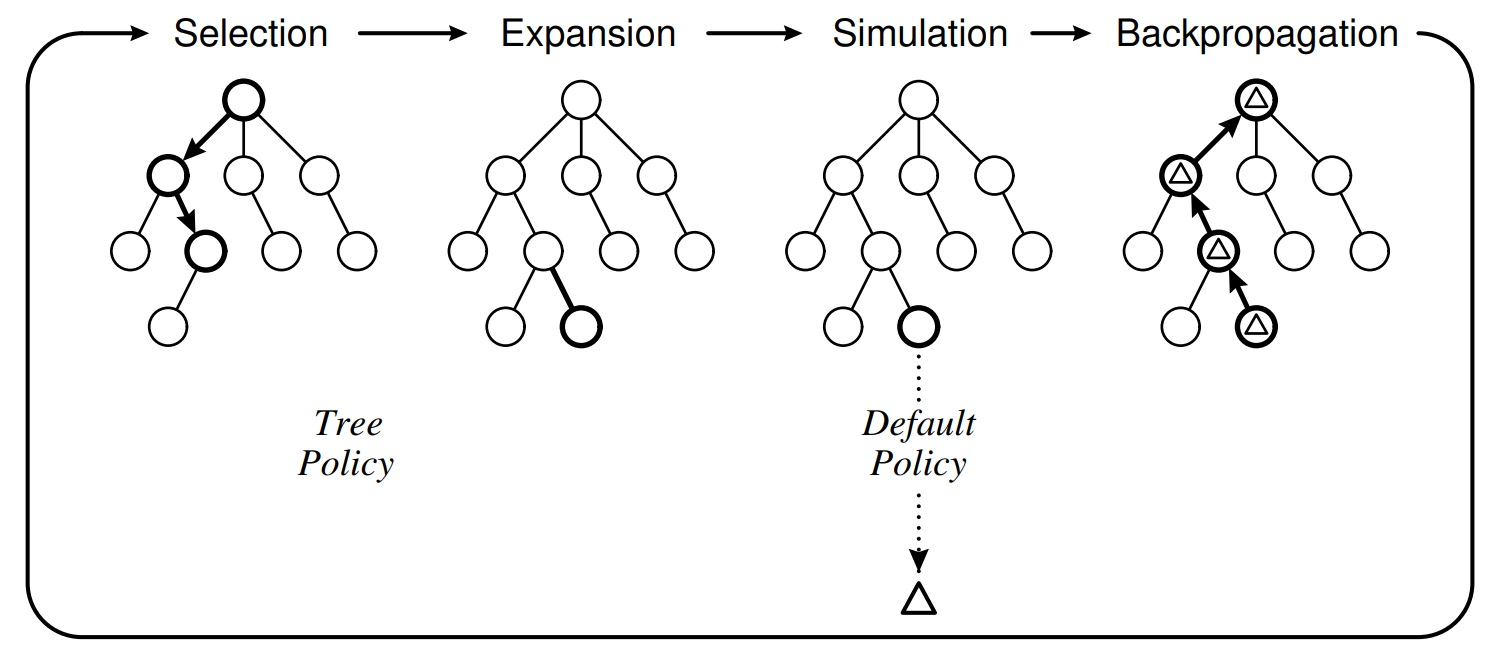
\includegraphics[width=\textwidth]{mcts-steps.jpg}
  \end{center}
  \caption{MCTS steps, credit to \cite{mcts-survey}}
  \label{fig:mcts-steps}
\end{figure}

\subsubsection{Selection}
Starting at the root node, select the child node by tree policy. Then recursively select child nodes through the tree until an ``expandable node'' is reached. A node is expandable if it represents a nonterminal state and has unvisited children (i.e. unexpanded).

\subsubsection{Expansion}
One (or more) child nodes are added to expand the tree, according to the available actions.

\subsubsection{Simulation (Rollout)}
A simulation is run from the new node(s) according to the default policy to produce an outcome.
\subsubsection{Backpropagation}
The simulation result is ``backed up'' (i.e. backpropagated) through the selected nodes to update their statistics.

\subsection{Exploration and exploitation}
Maintaining a balance between exploration and exploitation is an important part of implementing decision-making algorithms such as MCTS. During MCTS processes, all nodes have some chance of being randomly picked, which allows new decisions to be made so that new and better outcomes can be discovered. This is called exploration. At the same time, nodes that lead to a winning state will have a higher chance of being picked again in subsequent \glspl{playout}. This is called exploitation.

\subsection{UCB policy}
One of the most commonly used tree policies in MCTS is UCB (Upper Confidence Bound) \cite{RN2020}. As UCB is used in bandit problems, the process in selection phase can be modelled as a multi-armed bandit problem. A child node j is selected to maximize:

\begin{equation}
  \label{eq:UCB}
  \mathrm{UCB} = \overline{X}_j + 2C_p\sqrt{\frac{2\ln n}{n_j}} 
\end{equation}

where $n$ is the number of times a parent node has visited, $n_j$ is the number of times a child node has visited, $X_j$ is the average reward of the parent node, and $C_p > 0$ is a constant.

In (\ref{eq:UCB}), the two terms are the exploitation term and the exploration term, respectively. If a node has been explored a few times, the exploration term will be high as a denominator $n_j$. $C_p$ is a constant that balances between exploitation and exploration.

\subsection{Winning action selection} \label{winning-action}
MCTS continues to run four steps until the endgame condition is met or the computation budget is reached. Then, the action of the root node is selected by some criteria. \newline Browne says that there are four criteria for selecting winning action, based on their survey \cite{mcts-survey}:

\begin{enumerate}
  \item \textbf{Max}: Select the action that gives the most rewards.
  \item \textbf{Robust}: Select the action that visited the most. 
  \item \textbf{Max-Robust}: Select the action that has the most rewards and visits. If none exist, continue searching until they are found.
  \item \textbf{Secure}: Select the action that maximizes the lower confidence bound.
\end{enumerate}

% TODO: add citations to MCTS wikipedia

\subsection{MCTS with imperfect information game and uncertainty}

In a deterministic game, MCTS can generate future states in nodes that will be found when performing an action. This is called a Closed Loop MCTS \cite{Perez_Liebana_2015}. But when nondeterministic actions come into concern, such as rolling dice or drawing random cards, we can still use a Closed Loop MCTS to generate all available possible outcomes as states and play out each one. However, it should be noted that this approach will make the game tree grows exponentially. 

An approximate solution is to use an Open Loop MCTS. Open Loop MCTS only stores the statistics in the nodes, not the states. Instead, the state at a node must be computed by playing actions along the path from the root node to the current node. This way, a node does not represent a state but a series of actions executed starting from the initial state of the game.

To handle imperfect information and uncertainty, a game can be converted into a determistic game using \textit{determinization}, the process of sampling all possible outcomes of all chance events, making it fully observable \cite{mcts-survey}. For example, rolling dice can be simulated with a predetermined sequence of dice rolls.

% \section{Reinforcement learning} % TODO: 
% \cite{Reinforcement-Learning} Reinforcement learning (RL) is a popular method used in many branches of applications, including game optimization, industry automation, telecommunications, etc. There are five main elements of reinforcement learning:

% \begin{enumerate}
%   \item Agent: the player who makes a decision about what action to take
%   \item Environment: the world in which an agent takes actions
%   \item State: current situation of the agent
%   \item Reward: feedback from the environment
%   \item Policy: how agents make decisions
% \end{enumerate}

% \tikzstyle{block} = [rectangle, rounded corners, 
% minimum width=3cm, 
% minimum height=1cm,
% text centered, 
% draw=black]

% \tikzstyle{small_block} = [rectangle, rounded corners, 
% minimum width=2cm, 
% minimum height=1cm,
% text centered, 
% draw=black]

% \tikzstyle{dashed_one_side} = [draw, rectangle, dashed, inner sep=2em]

% \tikzstyle{arrow} = [draw, thick, -latex']

% \begin{figure}
%   \centering
%   \begin{tikzpicture}[node distance=2cm]
%     \node (env) [block] {Environment};
%     \node (agent) [block, below of=env] {Agent};
%     \node (poli) [small_block, below of=agent] {Policy};
  
%     \begin{scope}
%       \draw [arrow] (env)-- ($(env.east)-(-0.5,0)$) |- node[anchor=center, right, pos=0.225] {State, Reward} (agent);
%       \draw [arrow] (agent)--($(agent.west)-(0.5,0)$) |- node[anchor=center, left, pos=0.275] {Action} (env);
%       \draw [arrow] (poli) -- (agent);
%       \draw [arrow] (agent) -- (poli);
%     \end{scope}
%   \end{tikzpicture}
  
%   \caption{Reinforcement Learning Model}
%   \label{fig:rl-flow}
% \end{figure}

% The concept of this method is to use agents to learn in a reward-punishment environment. The reinforcement learning model is described in figure \ref{fig:rl-flow}. The goal of reinforcement learning is to learn a policy that maximizes the reward the agent will receive. At first, the agent will be given the objective they must achieve. At each timestep of learning, the agent will receive the current state and available actions. Then, the agent will decide what actions to take from the policy they have, moving to a new state. By using the reward function, the feedback is returned to the agent to tell how well they behave or how they take actions. The agent will use that feedback to update their policy and then take another action, repeating the process until the agent has reached its objectives.

% Reinforcement learning is different from supervised learning in that there is no correct answer in reinforcement learning; instead, the reinforcement agent decides how to carry out the given task. In supervised learning, the training data includes the answer key, so the model is trained with that answer.
 
%%%%%%

% \section{Second section}
% Section 2 text.

% \subsection{Subsection heading goes here}

% Subsection 1 text

% \subsubsection{Subsubsection 1 heading goes here}
% Subsubsection 1 text

% \subsubsection{Subsubsection 2 heading goes here}
% Subsubsection 2 text

% \section{Third section}
% Section 3 text. The dielectric constant\index{dielectric constant}
% at the air-metal interface determines
% the resonance shift\index{resonance shift} as absorption or capture occurs
% is shown in Equation~\eqref{eq:dielectric}:

% \begin{equation}\label{eq:dielectric}
% k_1=\frac{\omega}{c({1/\varepsilon_m + 1/\varepsilon_i})^{1/2}}=k_2=\frac{\omega
% \sin(\theta)\varepsilon_\mathit{air}^{1/2}}{c}
% \end{equation}

% \noindent
% where $\omega$ is the frequency of the plasmon, $c$ is the speed of
% light, $\varepsilon_m$ is the dielectric constant of the metal,
% $\varepsilon_i$ is the dielectric constant of neighboring insulator,
% and $\varepsilon_\mathit{air}$ is the dielectric constant of air.

% \section{About using figures in your report}

% % define a command that produces some filler text, the lorem ipsum.
% \newcommand{\loremipsum}{
%   \textit{Lorem ipsum dolor sit amet, consectetur adipisicing elit, sed do
%   eiusmod tempor incididunt ut labore et dolore magna aliqua. Ut enim ad
%   minim veniam, quis nostrud exercitation ullamco laboris nisi ut
%   aliquip ex ea commodo consequat. Duis aute irure dolor in
%   reprehenderit in voluptate velit esse cillum dolore eu fugiat nulla
%   pariatur. Excepteur sint occaecat cupidatat non proident, sunt in
%   culpa qui officia deserunt mollit anim id est laborum.}\par}

% \begin{figure}
%   \centering

%   \fbox{
%      \parbox{.6\textwidth}{\loremipsum}
%   }

%   % To include an image in the figure, say myimage.pdf, you could use
%   % the following code. Look up the documentation for the package
%   % graphicx for more information.
%   % \includegraphics[width=\textwidth]{myimage}

%   \caption[Sample figure]{This figure is a sample containing \gls{lorem ipsum},
%   showing you how you can include figures and glossary in your report.
%   You can specify a shorter caption that will appear in the List of Figures.}
%   \label{fig:sample-figure}
% \end{figure}

% Using \verb.\label. and \verb.\ref. commands allows us to refer to
% figures easily. If we can refer to Figures
% \ref{fig:walrus} and \ref{fig:sample-figure} by name in the {\LaTeX}
% source code, then we will not need to update the code that refers to it
% even if the placement or ordering of the figures changes.

% \loremipsum\loremipsum

% % This code demonstrates how to get a landscape table or figure. It
% % uses the package lscape to turn everything but the page number into
% % landscape orientation. Everything should be included within an
% % \afterpage{ .... } to avoid causing a page break too early.
% \afterpage{
%   \begin{landscape}
%   \begin{table}
%     \caption{Sample landscape table}
%     \label{tab:sample-table}

%     \centering

%     \begin{tabular}{c||c|c}
%         Year & A & B \\
%         \hline\hline
%         1989 & 12 & 23 \\
%         1990 & 4 & 9 \\
%         1991 & 3 & 6 \\
%     \end{tabular}
%   \end{table}
%   \end{landscape}
% }

% \loremipsum\loremipsum\loremipsum

% \section{Overfull hbox}

% When the \verb.semifinal. option is passed to the \verb.cpecmu. document class,
% any line that is longer than the line width, i.e., an overfull hbox, will be
% highlighted with a black solid rule:
% \begin{center}
% \begin{minipage}{2em}
% juxtaposition
% \end{minipage}
% \end{center}

% \section{\ifenglish%
% \ifcpe CPE \else ISNE \fi knowledge used, applied, or integrated in this project
% \else%
% ความรู้ตามหลักสูตรซึ่งถูกนำมาใช้หรือบูรณาการในโครงงาน
% \fi
% }

% อธิบายถึงความรู้ และแนวทางการนำความรู้ต่างๆ ที่ได้เรียนตามหลักสูตร ซึ่งถูกนำมาใช้ในโครงงาน

% \section{\ifenglish%
% Extracurricular knowledge used, applied, or integrated in this project
% \else%
% ความรู้นอกหลักสูตรซึ่งถูกนำมาใช้หรือบูรณาการในโครงงาน
% \fi
% }

% อธิบายถึงความรู้ต่างๆ ที่เรียนรู้ด้วยตนเอง และแนวทางการนำความรู้เหล่านั้นมาใช้ในโครงงาน
